\chapter{Stand der Dinge}
\label{Kapitel3}

Das vorliegende Kapitel widmet sich der Untersuchung des aktuellen Forschungsstands auf dem Gebiet der akustischen Vermessung von robotischen Schleifprozessen zur prädiktiven Wartung. Anschließend wird auf die spezifischen Herausforderungen und Möglichkeiten eingegangen, die die akustische Vermessung in robotergestützten Schleifanwendungen bietet.
    

\section{Analyse des Audiosignals}
%https://www.intechopen.com/chapters/74096

Wie bereits im Kapitel \ref{Kapitel2} vermittelt, werden Informationen aus Audiosignalen extrahiert, indem das vorliegende Audiosignal in den Frequenzbereich umgewandelt wird. Dafür werden die Methoden der Fourier-Transformation und der Wavelet-Transformation genauer betrachtet. Im Folgenden werden nun praktische Umsetzungen zu diesen Methoden aufgezeigt.

\subsection{Fast Fourier transform}

Angefangen bei der praktischen Umsetzung der Fourier-Transformation. Hierzu hat im Laufe der Zeit festgestellt, dass der ursprüngliche Algorithmus sehr komplex und zeitaufwendig ist und somit bei der praktischen Anwendung nicht effektiv eingesetzt werden kann. Aus diesem Grund haben sich zahlreiche Heuristiken Entwickelt, welche diese Berechnung schneller machen und dennoch gute Ergebnisse erzielen. Diese Heuristiken sind heutzutage allgemein als \ac{FFT} bekannt. \cite[155f.]{Meyer2000} Praktisch gesehen ist fast jede praktische Implementierung der \ac{FT} eigentlich eine \ac{FFT}. \cite[6]{Heckbert1995}

\paragraph{Cooley und Tukey}
   
Der \ac{FFT}-Algorithmus von Cooley und Tukey, oder auch Radix-2-Algorithmus genannt, ist der bekannteste Algorithmus für die schnelle Berechnung einer \ac{FT}, da er sowohl leicht zu implementieren ist, als auch konsistent sehr gute Ergebnisse liefert. \cite[156ff.]{Meyer2000} 
Dies erreicht der Algorithmus, indem er die \ac{DFT} direkt und nicht über Matrixmultiplikation berechnet. Der Trick dahinter ist die Nutzung von Rekursion. So wird die zu berechnende Matrix wieder und wieder in zwei Teile aufgeteilt, bis die Teile so klein sind, dass die Anwendung der \ac{DFT} nur geringfügig komplex ist. Die einzige Bedingung hierfür ist, dass die Anzahl der Objekte eine Zweierpotenz sein muss. \cite{Rabiner1969} Erreichbar ist dies aber mit einfachen 0-padding. \cite[41 ff.]{Aamir2005} Diese Implementierung alleine ist schon eine gültige \ac{FFT}, jedoch fehlt hierbei ein weiterer Trick, welcher den Algorithmus besonders macht. Dieser Trick sind sogenannte Butterfly-Diagramme. Diese Diagramme überwachen und sortieren die Elemente in jedem Zustand der \ac{FFT}. Sie sorgen dafür, dass die Listen, auf welchem die \ac{DFT} durchgeführt wird, Werte enthalten die nahe beieinander liegen, wodurch die Berechnung der DFT schneller durchgeführt werden kann. \cite[3ff.]{Burrus2009} \cite[7]{Heckbert1995} Dafür werden immer Approximationen von zwei Werte verglichen, weshalb der Algorithmus auch Radix-2-Algorithmus genannt wird.  Diese Sortierung reduziert am Ende die Komplexität mehr als sie selbst bei der Implementierung erzeugt, wodurch der Algorithmus effizienter wird. Auf die dahinter steckenden mathematischen Beweise wird in dieser Arbeit nicht weiter eingegangen.  Bei Interesse werden weiterführende Quellen empfohlen.  \cite[9f.]{Heckbert1995} \cite{Bekele2016}

Neben dem Algorithmus von Cooley und Tukey gibt es noch weitere Algorithmen, welche die \ac{DFT} durch Heuristiken weniger komplex berechnen. Die bekanntesten Vertreter hierbei sind Primfaktor-Algorithmen und die Chirp-z-Transformation. Im Allgemeinen zielen die Primfaktor-Algorithmen darauf ab die Anzahl an Multiplikationen während einer \ac{DFT} zu reduzieren, indem die Anzahl an Additionen erhöht wird. Da Additionen weniger komplexe mathematische Operationen sind, sinkt somit die Komplexität zur Berechnung der \ac{DFT}. \cite{Temperton1992} Die Chirp-z-Transformation oder auch Bluestein-FFT genannt, berechnet die \ac{DFT}, indem diese als komplexe Faltung betrachtet wird, welche stattdessen gelöst wird. Dadurch wird die Einschränkung, dass die Anzahl der Daten eine Zweierpotenz sein muss aufgehoben. \cite{Rabiner1969} Auf eine genauere Erläuterung dieser Alternativen und der mathematischen Grundlagen dahinter, wird in dieser Arbeit verzichtet, da wie an späterer Stelle genauer erläutert die für die Umsetzung genutzten Implementierungen auf dem Algorithmus von Cooley und Tukey beruhen.

\subsection{Kurzzeit-Fourier Transformation}
    
Wie bereits im Kapitel Grundlagen \ref{Kapitel2} erläutert ist einer der größten Nachteile der \ac{FT}, dass jegliche Informationen über die Zeit verloren geht. In Falle der Schleifanalyse bedeutet dies, dass nach der Anwendung der \ac{FT} auf eine Audiospur nicht erkennbar ist, wann in dieser Audiospur beispielsweise eine Anomalie auftritt, des Weiteren kann es auch passieren, dass die auftretende Anomalie in einem so kurzen Zeitabschnitt geschieht, sodass diese im letztendlichen Ergebnis des \ac{FT} völlig untergeht. Die einfachste Lösung hierzu ist, dass man die \ac{FT} nicht auf das ganze Audiosignal anwendet, sondern immer nur auf einen kleinen Teil. Dieser Algorithmus wird dann als \ac{STFT} bezeichnet, wobei die Umsetzung der \ac{FT} immer durch eine im letzten Kapitel \ref{Kapitel2} erläuterte \ac{FFT} stattfindet. \cite{Okumura2011}

\paragraph{Funktionsweise der Kurzzeit-Fourier-Transformation}
    
Grundsätzlich gesprochen funktioniert die \ac{STFT}, indem ein Teil-Zeitabschnitt festgelegt wird, auf welchem dann eine \ac{STFT} angewendet wird. Der Zeitabschnitt wird dann verschoben, dieses Vorgehen wird dann rekursiv weitergeführt, bis das ganze Audiosignal betarchtet wurde. Im Beispiel gesprochen heißt das, dass bei einem 10-sekündigen Audiosignal eine \ac{FFT} immer aus z.B. eine Sekunde angewendet wird. Die Ergebnisse dieser 10 \ac{FFT} werden anschließend zusammengefasst. \cite[69]{Kiencke2008}
Dieses Schrittweise ablaufen des Signals kann schon als \ac{STFT} betarchtet werden, jedoch gibt es viele Parameter, welche die \ac{STFT} beeinflussen können, um so das Ergebnis zu optimieren. So entstanden die Idee eines Fensters und des Versatzes. \cite[5f.]{Okumura2011} Ein Fenster besitzt hierbei eine feste Breite, welche dann auf den Zeitabschnitt des Signals gelegt werden kann, auf welchen eine \ac{FFT} durchgeführt werden soll. Die Wahl der Breite bestimmt die Genauigkeit des Ergebnisses, welche sich in Zeitgenauigkeit und Frequenzgenauigkeit aufteilen lässt. \cite{jacobsen2003} Diese Genauigkeiten können nie gleichzeitig hoch sein, dieses Problem ist in der Quantenmechanik auch als ,,Uncertainty Principle'' bekannt. \cite{uncertainty2024} Will man nun die Zeitgenauigkeit erhöhen, so  muss die Fenster-Größe verringert werden. Im Gegenzug sinkt jedoch die die Frequenzgenauigkeit. 
    
Der zweite Parameter einer \ac{STFT} ist der Versatz, dieser beschreibt wie weit das Fenster sich nach jeder Anwendung der \ac{FFT} verschiebt. Der Versatz wird typischerweise nun kleiner als das Fenster gewählt, sodass jeder Datenpunkt nicht nur einmal sondern mehrmals ausgewertet wird. Dieses mehrfache Auswerten jedes Datenpunktes erhöht zum einen die Genauigkeit des Ergebnisses und glättet zum anderen den Übergang zwischen den Ergebnissen zweier nachfolgender \ac{FFT}. Je kleiner der Versatz, desto höher ist jedoch auch der Berechnungsaufwand. \cite{jacobsen2003} Die Abbildung \ref{fig:hop-overlpa-fenster} zeigt die Anwendung solcher Fenster und des Versatzes im allgemeinen und die Abbildung \ref{fig:different-overlaps} zeigt die Auswirkung verschiedener Versetze auf ein Ergebnis.
    
    \begin{figure}[H]
        \centering
        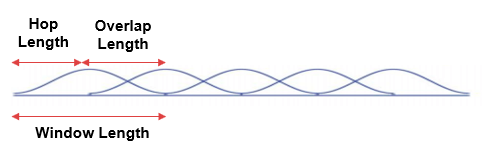
\includegraphics[width=0.5\linewidth]{images/hop-overlpa-fenster.png}
        \caption{Visualisierung des Fensters und des Versatzes \cite{hopAWindow}}
        \label{fig:hop-overlpa-fenster}
    \end{figure}
    
    \begin{figure}[H]
        \centering
        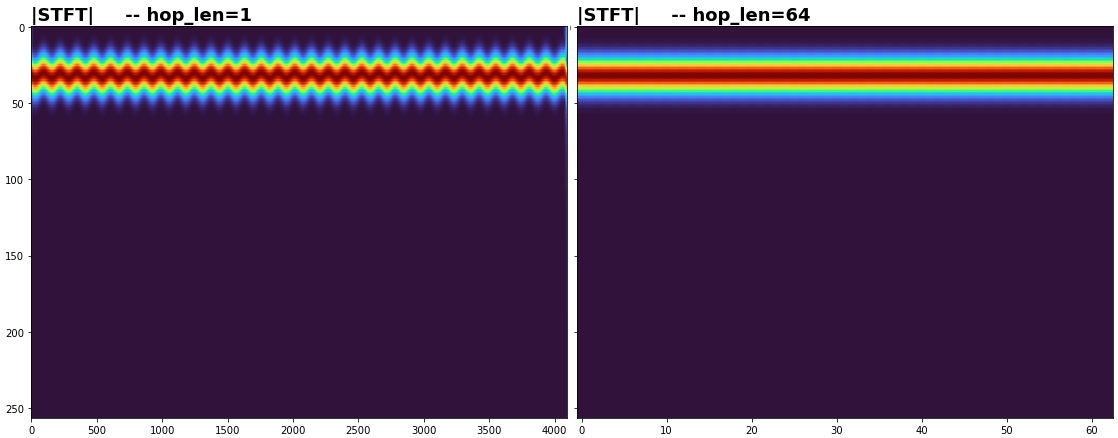
\includegraphics[width=0.5\linewidth]{images/different-overlaps.png}
        \caption{Auswirkungen verschiedener Versätze \cite{versätze}}
        \label{fig:different-overlaps}
    \end{figure}
    %https://dsp.stackexchange.com/questions/19311/stft-why-overlapping-the-window
    
Zusätzlich zu der Wahl des Versatzes lässt sich aber auch das Fenster anpassen. So kann das Fenster nicht nur eine Breite haben, sondern es kann zusätzlich eine Funktion gewählt werden, die die Daten innerhalb des Fensters manipuliert. Die einfachste Funktion spiegelt die zu analysierenden Daten 1zu1 wieder. Jedoch ist es auch möglich beispielsweise eine Funktion als Grundlage zu benutzen, welche die Daten, welche im Zentrum des Fensters liegen stärker gewichtet. Die Abbildungen \ref{fig:Veranschaulichung verschiedener Fenster und deren Frequenzspektren} zeigen verschiedene Beispiele solcher Fenster. 

    \begin{figure}[H]
        \centering
        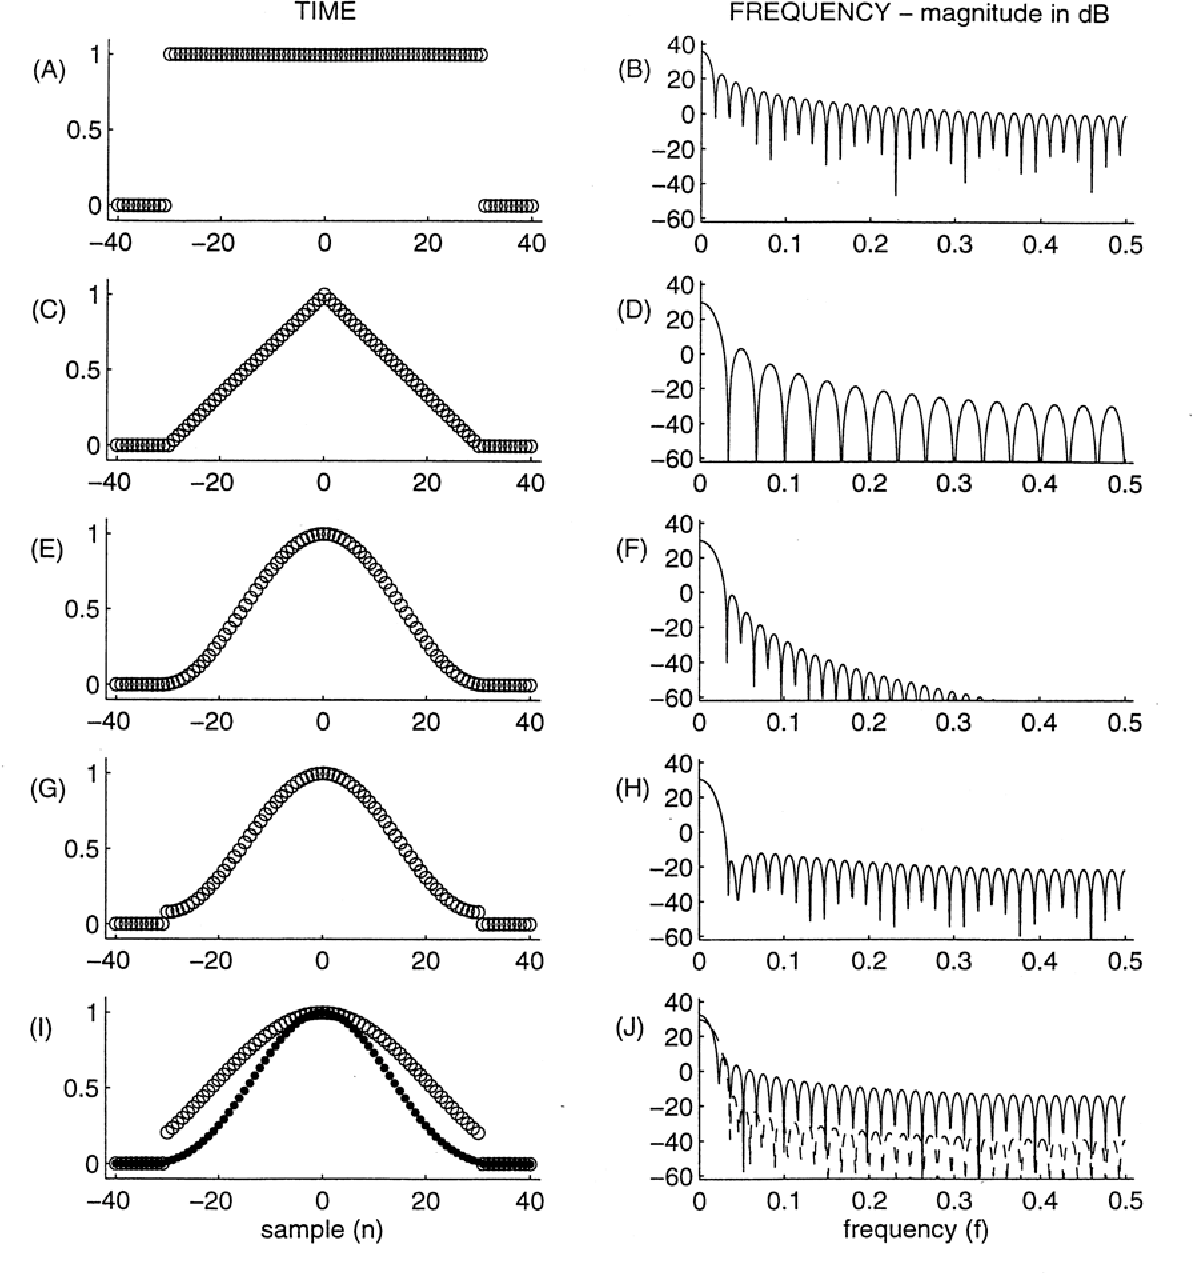
\includegraphics[width=0.5\linewidth]{images/Veranschaulichung verschiedener Fenster und deren Frequenzspektren.png}
        \caption{Veranschaulichung verschiedener Fenster und deren Frequenzspektren} \cite{windowFunctions}
        \label{fig:Veranschaulichung verschiedener Fenster und deren Frequenzspektren}
    \end{figure}
    
Der Vorteil der durch den in Abbildungen \ref{fig:Veranschaulichung verschiedener Fenster und deren Frequenzspektren} gezeigten Fenster entstehen dadurch, dass wie bereits zuvor erwähnt die am Rand des Fenster liegenden Datenpunkte durch die Wahl des Versatzes sowieso mehrfach analysiert werden und somit eine höhere Gewichtung im Endergebnis erhalten. Durch die stärkere Gewichtung der Zentralen Daten wird dem entgegengewirkt. Aus diesem Grund hat sich die Gaussian-Verteilung als gute Allgemeine Lösung etabliert, welche durch die Wahl der Standardabweichung auf den jeweiligen Versatz und zu lösendes Problem angewendet werden kann.
    
Zusammengefasst lässt sich festhalten, dass die Wahl der einzelnen Parameter stark von dem zu lösenden Problem abhängen. Durch die Notwendigkeit der Festlegung dieser Parameter entsteht auch das Problem, dass je nach Signalart oder Signallänge verschiedene Parameter zu verschiedenen Ergebnissen führen kann und die Wahl dieser Parameter somit einer hohen Komplexität unterliegen. So können die Parameter, welche gute Ergebnisse für ein Problem bei langen Signalen erzeugen schlechte Ergebnisse beim selben Problem und kurzen Signalen erzeugen. Kurz gesagt kann es sich als sehr schwierig herausstellen eine \ac{STFT} zu generalisieren, sei es auch nur für einen spezifischeren Anwendungsfall, wie die Analyse von Schleifgeräuschen. Inwiefern dieses Problem in diesem Fall besteht wird in der späteren Durchführung genauer erläutert, wenn tatsächlich mehrere verschiedene \ac{STFT} implementiert und ausgewertet werden.

\subsection{Kontinuierliche Wavelet-Transformation}

Die \ac{CWT} ist wie die \ac{STFT} eine Methode zur Analyse von Signalen. Wie bereits in \ref{ss:wavelet} beschrieben, bietet die \ac{WT} im Vergleich zur \ac{FT} den Vorteil, die zeitlichen Komponente der Signalen zu bewahren. 
Sie kommt an verschiedensten Bereichen zum Einsatz, wie zum Beispiel in der Meteorologie bei der Analyse von zyklischen Wetterphänomenen \cite{Torrence1999}.

\paragraph{Funktionsweise der Kontinuierlichen Wavelet-Transformation}

Bei der \ac{CWT} wird ein Signal mit einer skalierten und verschobenen Version eines sogenannten ,,Mother-Wavelet'' gefaltet. Beispiele für häufig verwendete Wavelets sind das in \ref{ss:wavelet} gezeigten Haar-Wavelet (siehe Abbildung \ref{fig:haar-wavelet}) welches durch Gleichung \ref{eq:haar} beschrieben wird und das Morlet-Wavelet (siehe Abbildung \ref{fig:morlet-wavelet}) welches durch \ref{eq:morlet} beschrieben wird. Die Transformation wird durch folgende Gleichung beschreiben \cite[92]{Schulte2019}:

\begin{equation}
W(a, b) = \int_{-\infty}^\infty x(t) \Psi^* \left( \frac{t - b}{a} \right) dt
\end{equation}

Hierbei stellt \(x(t)\) das zu analysierende Signal da und \(\Psi(t)\) das ,,Mother''-Wavelet. Mithilfe von \(a\) kann das Wavelet skaliert werden und mit \(b\) verschoben werden. 
Der Skalierungsparameter \(a\) variiert die Breite des Wavelets. Ein großer Skalar \(a\) entspricht dabei einer breiten Wavelet-Funktion und ermöglicht das Abtasten auf niedrigere Frequenzen. Dabei sinkt jedoch die Auflösung in der Zeit-Domäne. \cite{Torrence1998}

Der Parameter \(b\) gibt an, zu welchem Zeitpunkt die Analyse durchgeführt wird. Durch kontinuierliche Verschiebung des Wavelets entlang der Zeitachse kann die zeitliche Entwicklung einzelner Frequenzkomponenten des Signals verfolgt werden.

\paragraph{Beispielhafte Verwendung}

Um die Funktionsweise der \ac{CWT} zu veranschaulichen, betrachten wir zwei Beispiele, die anhand der folgenden Abbildungen dargestellt werden.

 \begin{figure}[H]
     \centering
            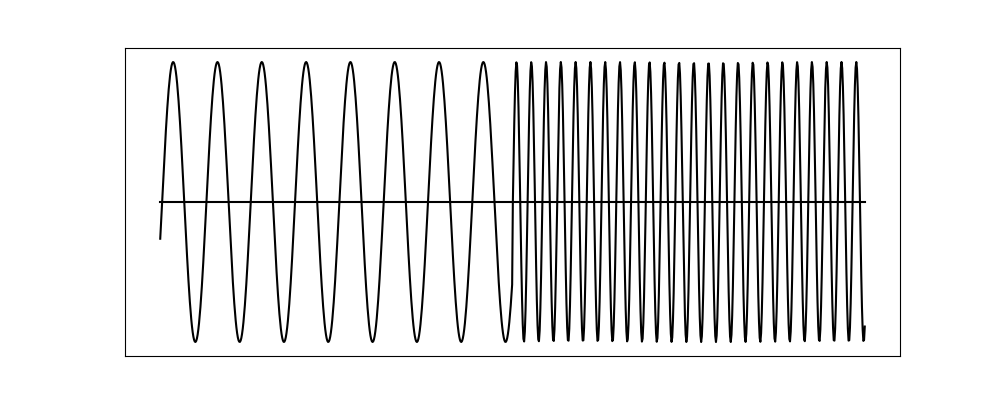
\includegraphics[width=0.9\linewidth]{images/aprupt_change_signal.png}
            \caption{Signal mit einer abrupter Frequenzänderung in der Mitte}
            \label{fig:aprupt_change_signal}
            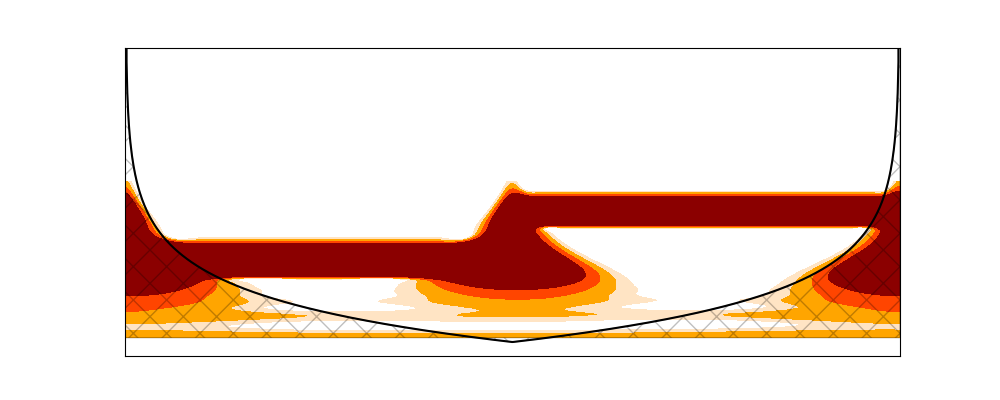
\includegraphics[width=0.9\linewidth]{images/aprupt_change_cwt.png}
            \caption[CWT Analyse eines Signals mit abrupter Frequenzänderung]{CWT Analyse des Signals von Abbildung \ref{fig:aprupt_change_signal}. Die Skalierung der y-Achse ist logarithmisch. Der schraffierte Bereiche stellen den so genannte ,,cone of influence'' da, in dem Randeffekte zu großen Einfluss haben} 
            \label{fig:aprupt_change_cwt}
        % \caption{Two pictures}
\end{figure}

Abbildung \ref{fig:aprupt_change_signal} zeigt ein Signal, das in der Mitte eine abrupte Frequenzänderung aufweist. Die zugehörige \ac{CWT}-Analyse ist in Abbildung \ref{fig:aprupt_change_cwt} dargestellt. Hier ist deutlich zu erkennen, dass die \ac{CWT} die zeitliche Position der Frequenzänderung erfasst. In der linken Hälfte der Analyse ist eine niedrige Frequenz dominant, während in der rechten Hälfte eine höhere Frequenz auftritt. Dies verdeutlicht die Fähigkeit der \ac{CWT}, sowohl zeitliche als auch frequenzielle Informationen des Signals präzise darzustellen.

\begin{figure}[H]   
     \centering
    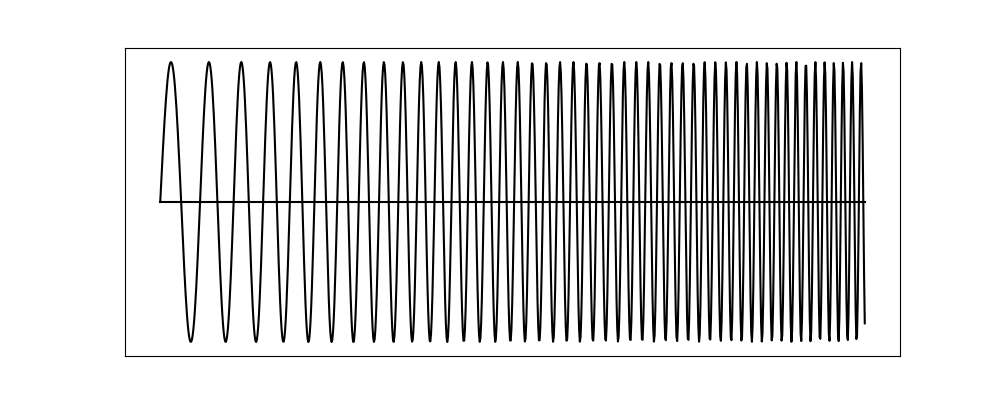
\includegraphics[width=0.9\linewidth]{images/continous_change_signal.png}
    \caption{Signal mit kontinuierlicher Frequenzänderung}
    \label{fig:continous_change_signal}   
    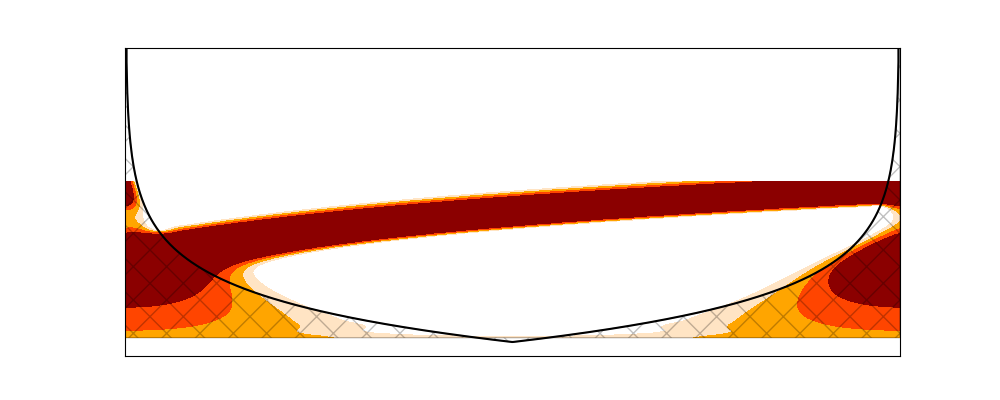
\includegraphics[width=0.9\linewidth]{images/continous_change_cwt.png}
    \caption[CWT Analyse eines Signals mit kontinuierlicher Frequenzänderung]{CWT Analyse des Signals von Abbildung \ref{fig:continous_change_signal}. Die Skalierung y-Achse ist logarithmisch. (Schraffierter Bereich siehe \ref{fig:aprupt_change_cwt})}
    \label{fig:continous_change_cwt}
% \caption{Two pictures}
\end{figure}

In Abbildung \ref{fig:continous_change_signal} sehen wir ein Signal mit einer kontinuierlichen Frequenzänderung. Die zugehörige \ac{CWT}-Analyse ist in Abbildung \ref{fig:continous_change_cwt} dargestellt. Hier zeigt die \ac{CWT}-Analyse eine kontinuierliche Änderung der Frequenz über die Zeit hinweg. Dies wird durch eine schrittweise Verschiebung des Frequenzbereichs in der Zeit-Frequenz-Darstellung deutlich. Diese Analyse ermöglicht es, den Verlauf der Frequenzänderungen im Signal über die Zeit präzise zu verfolgen.

Wie in den beiden Beispielen verdeutlicht wurde, bietet die \ac{CWT} Änderungen verschiedenster Art in Signalen identifizieren zu können. Somit bietet die \ac{CWT} ein vielseitiges Werkzeug, um zeitabhängige Besonderheiten in Signalen identifizieren und im Anschluss analysieren zu können.

\subsection{Signifikanztests}

Ein Problem, dass sich bei der Analyse mit Wavelets ergibt, ist das finden von signifikanten Ereignissen in der Zeit-Frequenz-Domäne, wie auch schon Lau in \cite[2401]{Lau1995} anmerkt. 

Dabei kann zwischen vier verschiedenen statistischen Signifikanztests unterschieden werden \cite{Schulte2019}:

\begin{enumerate}
    \item Point-wise tests
    \item Area-wise test
    \item Geometric test
    \item Cumulativ-area-wise tests
\end{enumerate}

Wir wollen im folgenden nur auf Point-wise und Area-wise tests eingehen.

\paragraph{Point-wise signifikance tests}
Bei Point-wise tests wird zuerst ein Signifikanzniveau ermittelt. Im Anschluss wird dann jeder Punkt mit diesem Signifikanzniveau verglichen um so konkrete Ereignisse zu erkennen.

Um Signifikanzniveaus für ein Waveletspektrum zu bestimmen, muss zunächst ein geeignetes Hintergrundspektrum gewählt werden, oft weißes Rauschen, mit gleichbleibender Leistung für alle Frequenzen. Ein weiteres häufig verwendetes Rauschen ist rotes Rauschen, bei dem die Leistung mit abnehmender Frequenz zunimmt. Diese Spektren dienen als Nullhypothese, gegen die das tatsächliche Spektrum verglichen wird. \cite[67f]{Torrence1998}

Wenn ein Peak im Waveletspektrum signifikant über dem Hintergrundniveau liegt, wird er als echtes Merkmal angenommen. So ist es möglich, Unterschiede zwischen wichtigen Ereignissen im Signal und zufälligen Schwankungen zu erkennen und Bereiche hoher statistischer Signifikanz zu identifizieren.

Wie Maraun und Kurths in \cite[511]{Maraun2004} hinweisen, haben Point-wise tests jedoch einige Nachteile:
So sind, um korrekte Signifikanzniveaus zu wählen oft Monte-Carlo Simulationen notwendig und es kann zu irreführenden Peaks kommen, welche die Auswertung verfälschen.

\paragraph{Area-wise signifikance-tests}

Area-wise signifikance-tests sind eine Erweiterung der Point-wise tests. Hierbei werden, wie beim Point-wise testing, alle Punkte mit einem zuvor ermittelten Signifikanzniveau verglichen. Zusätzlich dazu wird jedoch die Fläche der so entstandenen Flecken betrachtet \cite{Maraun2007}. Hierbei sind Flecken mit größerer Fläche statistisch signifikanter. Zusätzlich müssen diese Flecken eine gewisse Mindestgröße aufweisen, was dabei hilft, kleine, Falsch-Positive Flecken herauszufiltern. Dies hat jedoch zur Folge, das Area-wise signifikance-tests weniger sensitiv für kleine Ereignisse sind \cite{Schulte2016}. 

\section{Klassifizierung}

In folgenden Kapitel werden aktuelle Forschungen und wissenschaftliche Berichte im Bereich Klassifizierung mit KI vorgestellt. Diese Methoden sind vor allem wichtig, um zu sehen was bisher möglich ist. Eine KI Klassifizierung findet jedoch im Zuge der Arbeit nicht statt, vielmehr dient dieses Kapitel dazu, Klarheit darüber zu schaffen, wie es mit der Arbeit weiter gehen könnte. Dennoch ist es uns wichtig dieses Thema hier nicht zu kurz kommen zu lasse, da KI in vielen Bereichen immer mehr an Bedeutung gewinnt. Da wie in Kapitel \ref{Kapitel1} diese Arbeit eine Grundlage für weitere Arbeiten schaffen soll wird das Thema KI unabdingbar sein. 

\subsection{Verwendung von KI}
Die fortgeschrittene Analyse und Überwachung von Schleifprozessen mittels akustischer Daten stellt einen signifikanten Fortschritt in der Fertigungstechnologie dar, insbesondere durch die Anwendung von maschinellem Lernen und speziell tiefen neuronalen Netzwerken. Die Fähigkeit, aus dem kontinuierlichen Strom von Maschinengeräuschen präzise und nützliche Informationen zu extrahieren, hat weitreichende Implikationen für die Effizienz und Zuverlässigkeit industrieller Fertigungsprozesse. Maschinelles Lernen, insbesondere durch den Einsatz von Convolutional Neural Networks (CNNs), bietet eine effektive Lösung für die automatisierte Erkennung und Klassifizierung von Zustandsmerkmalen der Maschine basierend auf akustischen Signalen.

Neuronale Netzwerke sind besonders wertvoll in dieser Anwendung, da sie fähig sind, aus großen Datenmengen von Audiosignalen Muster zu erkennen und zu lernen, die für das menschliche Ohr nicht offensichtlich sind. Diese Fähigkeit, tiefergehende Einsichten aus den Audiodaten zu gewinnen, ohne auf vordefinierte Heuristiken oder manuell codierte Merkmale angewiesen zu sein, stellt einen Paradigmenwechsel dar. Durch Training mit umfangreichen Datensätzen können diese Modelle lernen, subtile akustische Unterschiede zu identifizieren, die auf spezifische Schleifzustände hinweisen. Dies verbessert nicht nur die Präzision in der Überwachung, sondern auch die Reaktionsfähigkeit des Produktionsprozesses, indem Anpassungen in Echtzeit ermöglicht werden, um optimale Betriebsbedingungen zu gewährleisten.


\subsection{Forschungsbeispiele und ihre Bedeutung}

In ihrer bahnbrechenden Studie \cite{Yang2019} untersuchten Yang und Rai die Anwendung von Convolutional Neural Networks (CNNs) zur akustischen Diagnostik von Maschinen mittels ,,Machine Auscultation'', analog zur medizinischen Auskultation, bei der Geräusche von Organen zur Diagnose genutzt werden. Ihre Forschung zielte darauf ab, abnormale Geräusche und Schwingungen, die während des Schleifprozesses auftreten, zu identifizieren und zu klassifizieren, speziell das Phänomen des Chatterns.

Das Team setzte CNNs ein, um die komplexen akustischen Signale, die von CNC-Maschinen während des Betriebs erzeugt werden, zu analysieren. Die Herausforderung bestand darin, aus den hochdimensionalen und oft verrauschten Daten nutzbare Informationen zu extrahieren. Die Forscher entwickelten ein System, das in der Lage war, aus den akustischen Daten zu lernen und diese zu verarbeiten, wodurch eine Echtzeit-Überwachung und -Analyse des Maschinenzustands ermöglicht wurde.

Die Ergebnisse von Yang und Rai zeigten, dass ihre CNN-basierten Modelle eine deutlich höhere Genauigkeit bei der Erkennung von Maschinenanomalien erreichen konnten als traditionelle Methoden. Besonders hervorzuheben ist die Fähigkeit des Modells, Chattern zu erkennen und zu klassifizieren, was zu einer signifikanten Verbesserung der Produktqualität und einer Reduzierung von Ausfallzeiten führen kann. Die Genauigkeit und Effizienz ihres Ansatzes wurde durch umfangreiche Tests und Validierungen bestätigt, wobei die Modelle eine bemerkenswerte Fähigkeit zur Unterscheidung zwischen normalen und abnormalen Betriebszuständen zeigten.

Die Studie von Cheng et al. \cite{Cheng2018} fokussierte sich auf die innovative Anwendung von Deep Convolutional Neural Networks (DCNNs) zur Zustandsüberwachung von Schleifbändern mittels akustischer Daten, die während des Schleifprozesses gesammelt wurden. Diese Forschungsarbeit verdeutlicht, wie DCNNs erfolgreich eingesetzt werden können, um den Verschleißzustand von Schleifwerkzeugen zu analysieren und vorherzusagen.

Cheng et al. entwickelten ein Modell, das darauf trainiert wurde, spezifische akustische Signaturen zu erkennen, die mit verschiedenen Verschleißgraden der Schleifbänder korrelieren. Durch das Training des Netzwerks mit einer umfangreichen Sammlung von Schleifgeräuschen konnten die Forscher eine hohe Genauigkeit in der Vorhersage des Werkzeugzustandes erreichen. Die Ergebnisse zeigten, dass ihr Modell eine Klassifizierungsgenauigkeit von 82,2\% und eine Präzision von 0,863 erzielte, was signifikant über den Fähigkeiten traditioneller Überwachungsmethoden liegt.

Die Anwendung von DCNNs ermöglichte eine detaillierte und zuverlässige Analyse der akustischen Daten, die während des Schleifens erfasst wurden. Diese Technologie bot nicht nur eine effektive Methode zur Vorhersage des Werkzeugverschleißes, sondern auch die Möglichkeit, Wartungsarbeiten präziser zu planen und durchzuführen, wodurch die Lebensdauer der Werkzeuge verlängert und die Produktionskosten gesenkt werden konnten.

In ihrer wegweisenden Studie untersuchten Liu et al. \cite{Liu2022} die Anwendung von Deep Convolutional Neural Networks (DCNNs) zur Klassifizierung von Fehlern in der vibrationsbasierten kontinuierlichen Zahnraderzeugung. Die Forschungsarbeit verdeutlicht, wie durch den Einsatz von fortgeschrittenen maschinellen Lernverfahren, insbesondere DCNNs, präzise und effiziente Überwachungsmethoden entwickelt werden können, die direkt auf die Vibrationsdaten angewendet werden, die während des Schleifprozesses entstehen.

Die Studie zielte darauf ab, nicht nur die Fehler während des Schleifprozesses zu identifizieren, sondern auch die spezifischen Bedingungen, unter denen diese Fehler auftreten, genau zu bestimmen. Dies wurde durch die Analyse der Vibrationsmuster erreicht, die mittels Sensoren erfasst wurden. Die DCNNs wurden dabei genutzt, um diese komplexen Muster zu dekodieren und in verwertbare Informationen umzuwandeln, die zur Fehlerdiagnose und Prozessoptimierung beitragen.

Die Forschungsergebnisse zeigten, dass die angewendeten Modelle in der Lage waren, mit einer beeindruckenden Genauigkeit von 95,83\% zu klassifizieren. Dies unterstreicht die Potenziale von DCNNs in der präzisen Fehlererkennung und der Minimierung von Produktionsausfällen durch frühzeitige Fehlererkennung. Zusätzlich wurden Grad-CAM-Visualisierungen verwendet, um die Entscheidungsfindung der Netzwerke zu illustrieren. Diese Visualisierungen ermöglichten es den Forschern und Praktikern, die spezifischen Merkmale innerhalb der Vibrationsdaten zu verstehen, die zu einer genauen Klassifizierung führten.

Die Studie von Nakai et al. \cite{Nakai2015} konzentrierte sich auf die Bewertung von neuronalen Modellen zur Schätzung des Werkzeugverschleißes beim Schleifen von Hochleistungskeramik. Vier verschiedene Arten von neuronalen Netzwerken, darunter auch tiefgehende neuronale Netzwerke (Deep Neural Networks), wurden untersucht, um deren Effektivität in der präzisen Vorhersage des Werkzeugzustands zu bewerten. Die Ergebnisse dieser Forschung zeigten, dass diese neuronalen Modelle fähig sind, aus den akustischen Daten während des Schleifprozesses wesentliche Informationen zu extrahieren. Diese Informationen sind entscheidend, um nicht nur den Verschleißzustand der Werkzeuge zu überwachen, sondern auch um die Prozesseffizienz zu optimieren und die Wartungskosten zu minimieren. Die Studie demonstrierte, wie maschinelles Lernen effektiv zur Überwachung und Verbesserung der Fertigungsprozesse eingesetzt werden kann, insbesondere in der anspruchsvollen Umgebung der Keramikverarbeitung .

\subsection{Zusammenfassung}

Die vielversprechendsten Methoden für die Klassifizierung im Bereich der Schleifprozessüberwachung sind \acp{CNN} und \acp{DCNN}. Diese Technologien haben gezeigt, dass sie hochdimensionalen und verrauschten akustischen Daten präzise analysieren können, um Anomalien und Zustände von Maschinen zu identifizieren. \acp{CNN}, wie in der Studie von Yang und Rai \cite{Yang2019}, und \acp{DCNN}, wie von Cheng et al. \cite{Cheng2018} und Liu et al. \cite{Liu2022} untersucht, bieten eine hohe Genauigkeit bei der Erkennung und Klassifizierung von Maschinenzuständen und -fehlern. Sie sind in der Lage, subtile akustische Unterschiede und komplexe Vibrationsmuster zu erkennen, was die Überwachung und Prozessoptimierung in der industriellen Fertigung signifikant verbessert. Trotz ihrer hohen Effizienz und Genauigkeit können diese Methoden jedoch nicht innerhalb dieser Arbeit verwendet werden. Die Gründe dafür liegen in der Komplexität und dem Umfang der Implementierung dieser Technologien, die über den Rahmen der aktuellen Arbeit hinausgehen. Es fehlen zudem die erforderlichen Datenmengen, um solche Modelle effektiv zu trainieren und einzusetzen.
In späteren Abschnitten der Arbeit wird erläutert, warum KI-Methoden nicht angewendet werden konnten und welche spezifischen Bedingungen und Anforderungen für deren erfolgreichen Einsatz erfüllt sein müssen. Dies wird dazu beitragen, Klarheit darüber zu schaffen, wie zukünftige Arbeiten auf dieser Grundlage weiterentwickelt werden können.
    
    
    
%%%%%%%%%%%%%%%%%%%%%%%%%%%%%%%%%%%%%%%%%%%%%%%%%%%%%%%%%%%%%%%%%%%%%%%%%%%%%%%
\endinput
%%%%%%%%%%%%%%%%%%%%%%%%%%%%%%%%%%%%%%%%%%%%%%%%%%%%%%%%%%%%%%%%%%%%%%%%%%%%%%%
